\section{Calibration des observations photométriques}
% Description des étapes du traitement et discussion de leurs effets.
Maintenant que nous avons rapidement introduit les paramètres de notre capteur CCD ainsi que de nos acquisitions, nous allons pouvoir présenter les différentes étapes nécessaire à la calibration de nos mesures photométriques. En effet, nous avons précédemment relié flux mesuré et magnitude, or ce flux dépend de nombreux facteurs que nous devons déterminer, en commençant par les critères qui vont définir la détection des sources présentes sur notre image. Notons ici rapidement que comme nous l'avons évoqué précédemment, nous avons travaillé avec deux types de filtres différents, or ceux-ci n'ayant pas d'impact sur le choix des paramètres de calibration en eux-mêmes, nous parlerons par la suite des données obtenues avec le filtre r puis nous utiliserons les mêmes paramètres pour le filtre g.

\subsection{Critères de détections}
Les critères de détection qui sont utilisés pour détecter des sources sur une image CCD dépendent en partie de l'outil utilisé. Dans notre cas, nous effectuons cette détection à l'aide de la librairie Python \textit{Photutils}, et celle-ci prend comme arguments la largeur à mi-hauteur, le pic maximum et le seuil de détection. \\

Premièrement, la largeur à mi-hauteur (ou FWHM de l'anglais Full Width at Half Maximum) permet de caractériser l'étalement des sources sur le CCD, et est liée à la fonction d'étalement du point. Pour la déterminer, nous pouvons regarder une étoile avec un excellent rapport signal/bruit (voir Figure \ref{fwhm}) et procéder à un ajustement Gaussien, puis déduire sa valeur des paramètres de ce dernier. La rondeur étant dans notre cas proche de 1, nous la considérons égale en $x$ et en $y$. Nous avons ainsi déterminé \text{FWHM=1.95} pixels.\\

Fixons maintenant le pic maximum, soit le critère de saturation: nous voyons sur la Table \ref{CCD} que la capacité maximale de notre capteur est de $10 ^{5} e-$, soit environ $65000$ ADU. Nous avons choisi de définir ce critère à $50 000$ ADU, car nous avons très peu de sources au-delà de cette valeur, nous en excluons donc une faible quantité tout en étant sûr d'être suffisamment loin du niveau de saturation du capteur. \\



Finalement, le dernier critère de détection à considérer est celui du "seuil", soit la valeur à partir de laquelle un pixel sera considéré comme une source. Une valeur trop proche de celle du fond de ciel signifie que l'on considérera par erreur des pixels chauds ou de simples variations du fond, tandis qu'une valeur trop haute implique simplement moins d'étoiles détectées, ce paramètre peut donc dans notre cas être utilisé pour faire varier le nombre de sources. En jouant sur ce paramètre, nous l'avons fixé arbitrairement à $100$ fois la valeur du fond de ciel, de manière à détecter un nombre de source suffisant pour effectuer une bonne calibration sans avoir de risque de détecter de "faux positifs".

\subsection{Méthodes d'annulation du fond de ciel\label{méthodes fond}}%
Discutons maintenant de la méthode que nous allons utiliser pour déterminer la valeur du fond de ciel de notre image. Nous avons à notre disposition deux méthodes, une méthode globale et une locale. Comme leur nom l'indique, la méthode globale consistera à regarder le fond à l'échelle de toute notre image, tandis que la méthode locale regardera le fond de ciel au voisinage de chacune de nos sources. Dans ces deux cas, nous nous intéresserons à la médiane des données, car elle plus robuste que la moyenne aux variations induites par les forts pics d'intensité des sources, ceux-ci étant concentrés sur une quantité limité de pixels à l'échelle de notre image.

\begin{figure}[h]
     \centering
     \begin{subfigure}[b]{0.42\textwidth}
         \centering
         \includegraphics[width=1\textwidth]{fig/bg corr.pdf}
         \caption{Correction du flux reçu pour une source quelconque en fonction du rayon d'ouverture}
         \label{subfig:bgcorr}
     \end{subfigure}
    \hfill
         \begin{subfigure}[b]{0.38\textwidth}
             \centering
              \includegraphics[width=1\textwidth]{fig/local global.pdf}
             \caption{Valeur du fond de ciel calculée pour chaque sources détectées}
             \label{subfig:localglobal}
         \end{subfigure} 
      \caption{Confrontation des deux méthodes d'annulation du fond de ciel}
       \label{fig:localglobal}
\end{figure}

\noindent Lorsque nous parlerons de rayon d'ouverture, nous parlerons à chaque fois du rayon du masque de l'étoile, cependant la méthode d'annulation locale nécessite de définir un rayon intérieur et extérieur pour le masque appliqué autour de chaque sources. Pour déterminer ce dernier, nous avons dans un premier temps corrigé le flux du fond de ciel globalement comme on peut le voir en Figure \ref{subfig:bgcorr}, puis à partir de cela nous avons déterminé qu'au delà d'un rayon d'ouverture d'environ trois pixels, nous ne semblions plus recevoir de flux des sources en elle-même, et ce quelque soit la source considérée (nous pouvons observer pour cela le flux corrigé pour des étoiles différentes et observer que le profil est constant à travers les sources, voir Figure \ref{annexe flux}). Ainsi, nous avons prit de manière relativement arbitraire un masque de rayons $r _{int}=4\text{pix}$ et $r _{ext}=6 \text{pix}$ pour le fond de ciel autour de nos sources. L'idée est d'avoir un échantillon suffisamment grand afin que les statistiques sur celui-ci soient pertinente, tandis qu'un masque trop grand augmente les chances de capter une autre source et non pas seulement le fond de ciel. \\

\noindent Pour finir sur l'annulation du fond de ciel, nous pouvons comparer la valeur de fond produite par ces deux méthodes pour chaque sources que nous avons détectée, ce qui est visible en Figure \ref{fig:localglobal}, où nous constatons que la valeur estimée localement oscille autour de la valeur globale, sauf pour certaines sources où celui-ci est clairement sur-évalué, ce qui correspond donc au cas décrit précédemment où une autre source a été prise en compte par le masque de ciel. Nous sources étant triées par valeur d'intensité maximale de pic, nous constatons également que pour les étoiles avec les pics les plus importants, la valeur du fond de ciel semble drastiquement augmenter. Dans la suite de nos discussion sur les paramètres de calibration, nous utiliserons une méthode de calibration globale, puis nous comparerons l'impact de ces deux méthodes sur la calibration photométrique. 


\subsection{Rayon d'ouverture optimal}

Nous l'avons rapidement abordé, le rayon d'ouverture est le paramètre le plus important à déterminer pour des mesures de photométrie d'ouverture, car celui-ci a un impact sur le flux mesuré et donc la magnitude, mais également le rapport signal/bruit de notre source, il est ainsi crucial de le fixer rigoureusement afin de calibrer avec précision notre zéro. Traditionnellement, ce rayon est exprimé comme un multiple de la FWHM, car il peut se déterminer selon la PSF de notre image, or dans notre cas nous utiliserons des méthodes "expérimentales" pour le fixer, cela a donc moins de sens, car nous balayerons toutes les valeurs possibles quoiqu'il arrive. Nous avons donc choisi de conserver cette convention de $R=r*\text{FWHM}$ avec $R$ le rayon d'ouverture et $r$ le facteur sur la FWHM et ainsi lorsque nous parlerons de rayons d'ouverture dans la suite du rapport nous parlerons de $r$. 
\subsubsection{Notion de rapport signal/bruit\label{Label}}%
Avant de présenter les différentes méthodes que nous avons utilisées pour déterminer ce rayon d'ouverture, introduisons rapidement la notion de rapport signal/bruit. En effet nous avons précédemment évoqué les sources de bruit d'un CCD, et fin de quantifier les électrons constituants le bruit de nos mesure nos introduisons donc la notion de rapport signal/bruit (RSB), qui quantifie la portion de notre mesure qui correspond réellement à des photons émis par les sources que nous observons. Il s'exprime comme:

\[\text{RSB}=\frac{N _{*}}{\sqrt{N _{*}+n _{pix}(N _{S}+N _{D} + N _{R}^2)}}\]

\noindent Avec $N _{*}$ le flux mesuré sur la source, $n _{pix}$ le nombre de pixels utilisés pour la mesure, $N _{S}$ la valeur du fond de ciel, $N _{D}$ le bruit d'obscurité (le courant d'obscurité multiplié par le temps d'exposition) et enfin $N _{R}$ le bruit de lecture. Ces informations seront tirés de la Table \ref{CCD} 
\subsubsection{Critère RSB sur chaque étoile\label{Label}}%
Nous pouvons maintenant décrire les trois méthodes dont nous allons discuter pour déterminer le rayon d'ouverture optimal, à commencer par un critère simple: étant donné que plus le RSB est élevé plus l'information mesurée provient effectivement de la source étudiée, nous allons chercher à faire varier le rayon d'ouverture pour chaque étoile détectée et chercher la valeur pour laquelle le RSB est maximal, ainsi nous travaillerons avec le signal le plus propre possible pour chaque sources.

\begin{figure}[h]
        \centering
        \includegraphics[width=0.4\linewidth]{fig/snr all.pdf}
        \caption{Rapport signal/bruit en fonction du rayon d'ouverture pour différentes étoiles}
        \label{rsb all}
\end{figure}

\noindent Comme nous pouvons nous y attendre à partir de son expression, nous constatons en Figure \ref{rsb all} que tant que le rayon d'ouverture est assez faible, l'augmenter revient à considérer d’avantages de photons provenant de la source, tandis qu'au-delà d'un certaine valeur (proche de la valeur où l'on atteint l'asymptote du flux en Figure \ref{subfig:bgcorr}), nous ne recevons plus que des photons du fond de ciel ce qui considérant la correction que nous avons effectuée revient donc à augmenter le bruit. Le rayon optimal, bien que semblant varier assez faiblement, n'est pas le même pour toutes les sources que nous considérons, ainsi il paraît pertinent d'établir un rayon différent pour chaque étoile, et nous reviendrons sur cette pertinence lorsque nous étudierons l'impact de ce choix sur la précision de la calibration. 
\subsubsection{Critère du RSB le plus faible\label{Label}}%
Un autre raisonnement que nous pouvons mener pour déterminer le rayon d'ouverture optimal est le suivant: étant donné que nous pouvons faire l'approximation que le RSB augmente avec la valeur de pic (cela n'est pas linéaire, cependant sur le nombre de sources avec lequel nous travaillons et les variations de RSB en jeu, c'est une approximation suffisante), nous pouvons alors chercher à trouver le rayon optimal d'une étoile avec une faible valeur de pic et utiliser cette valeur pour toutes nous sources. Si l'on cherche à avoir un critère fixe sur chaque étoiles, cette méthode permet de s'assurer que nous regardons le scénario où les variations relative (à sa valeur maximum) du RSB sont les plus importantes, transposer ce rayon aux autres étoiles aura donc moins d'impact sur leur RSB que si nous utilisions un critère sur l'étoile avec le meilleur RSB.

\subsubsection{Méthode d'optimisation Flux-RSB\label{fluxrsb}}%

Finalement, la dernière méthode que nous avons considérée pour fixer le rayon optimal d'ouverture est une méthode cherchant à trouver le point optimal en prenant en compte à la fois RSB et flux. Si l'on normalise le flux et le RSB, nous pouvons établir un critère sur les deux paramètres, car si l'on considère uniquement le RSB, on constate que la quantité de flux correspondant au rayon optimal n'est pas la valeur asymptotique, une partie des photons provenant de l'étoile n'est donc pas mesurée, ainsi l'idée est de trouver le point maximisant le RSB le plus proche de la valeur maximale du flux corrigé, ce qui n'a du sens que si l'on considère ces deux grandeurs normalisées.

\vspace{12\baselineskip}
\begin{figure}[h]
        \centering
        \includegraphics[width=0.4\linewidth]{fig/snr-flux.pdf}
        \caption{RSB et flux en fonction du rayon d'ouverture pour une source quelconque}
        \label{gsnrflux}
\end{figure}


\noindent On observe en Figure \ref{gsnrflux} que le rayon optimal obtenu est supérieur à celui obtenu par la méthode précédente et augmente la fraction totale du flux mesurée. Cette méthode est d'autant moins robuste face aux sources qui seraient très proches les unes de autres comme dans le cas d'étoiles binaires car on commence très vite à recevoir des photons de la seconde étoile et cela "casse" la normalisation.
\subsection{Impact de chaque méthodes sur la calibration\label{Label}}%
\noindent Finalement, nous allons calculer la constante $B$ pour chaque source et moyenner l'ensemble des valeurs obtenues pour obtenir notre zéro à l'écart-type près. Regardons l'impact qu'ont les différentes méthodes de détermination du rayon optimal d'ouverture sur l'incertitude associée à la calibration du zéro, et ce pour un même jeu d'étoiles.


\begin{figure}[h]
     \centering
     \begin{subfigure}[b]{0.4\textwidth}
         \centering
         \includegraphics[width=1\textwidth]{fig/incert.pdf}
         \caption{Avant correction}
         \label{subfig:incert}
     \end{subfigure}
     \hfill
          \begin{subfigure}[b]{0.4\textwidth}
              \centering
              \includegraphics[width=1\textwidth]{fig/incert corr.pdf}
              \caption{Après correction}
              \label{subfig:incert corr}
          \end{subfigure}
          
      \caption{Incertitude sur B en fonction du nombre d'étoiles utilisées pour la calibration}
       \label{fig:incert}
\end{figure}

En Figure \ref{fig:incert}, les sources sont triées par valeur de pic décroissante, toujours en approximant cela veut dire que l'on considère globalement les étoiles avec le meilleur RSB en premier puis les moins bon rapports signal/bruit tandis que le nombre d'étoiles considérées augmente. Aussi, il est important de relever qu'en Figure \ref{subfig:incert}, on observe de forts pics d'augmentation de l'incertitude sur B, qui correspondent en réalité au scénario que l'on a déjà précédemment évoqué, notre méthode de calcul de la magnitude est très peu robuste dans le cas de sources trop proches, car nous n'avons pas de moyen de déterminer de quelle sources les photons mesurés proviennent. Afin d'éviter ces écarts, nous appliquons le critère de correction suivant: si l'ajout d'un étoile au jeu de calibration augmente l'incertitude de B au-delà de l'écart-type de l'ensemble des incertitudes, celle-ci est ignorée pour la calibration. Cela exclu environ une vingtaine d'étoiles, et mène à ce que l'on observe en Figure \ref{subfig:incert corr}, à partir de laquelle nous fixerons la valeur finale du zéro, à partir donc du nombre d'étoiles utilisé pour la calibration minimisant l'erreur sur ce dernier. 

\begin{figure}[h]
     \centering
     \begin{subfigure}[b]{0.3\textwidth}
         \centering
         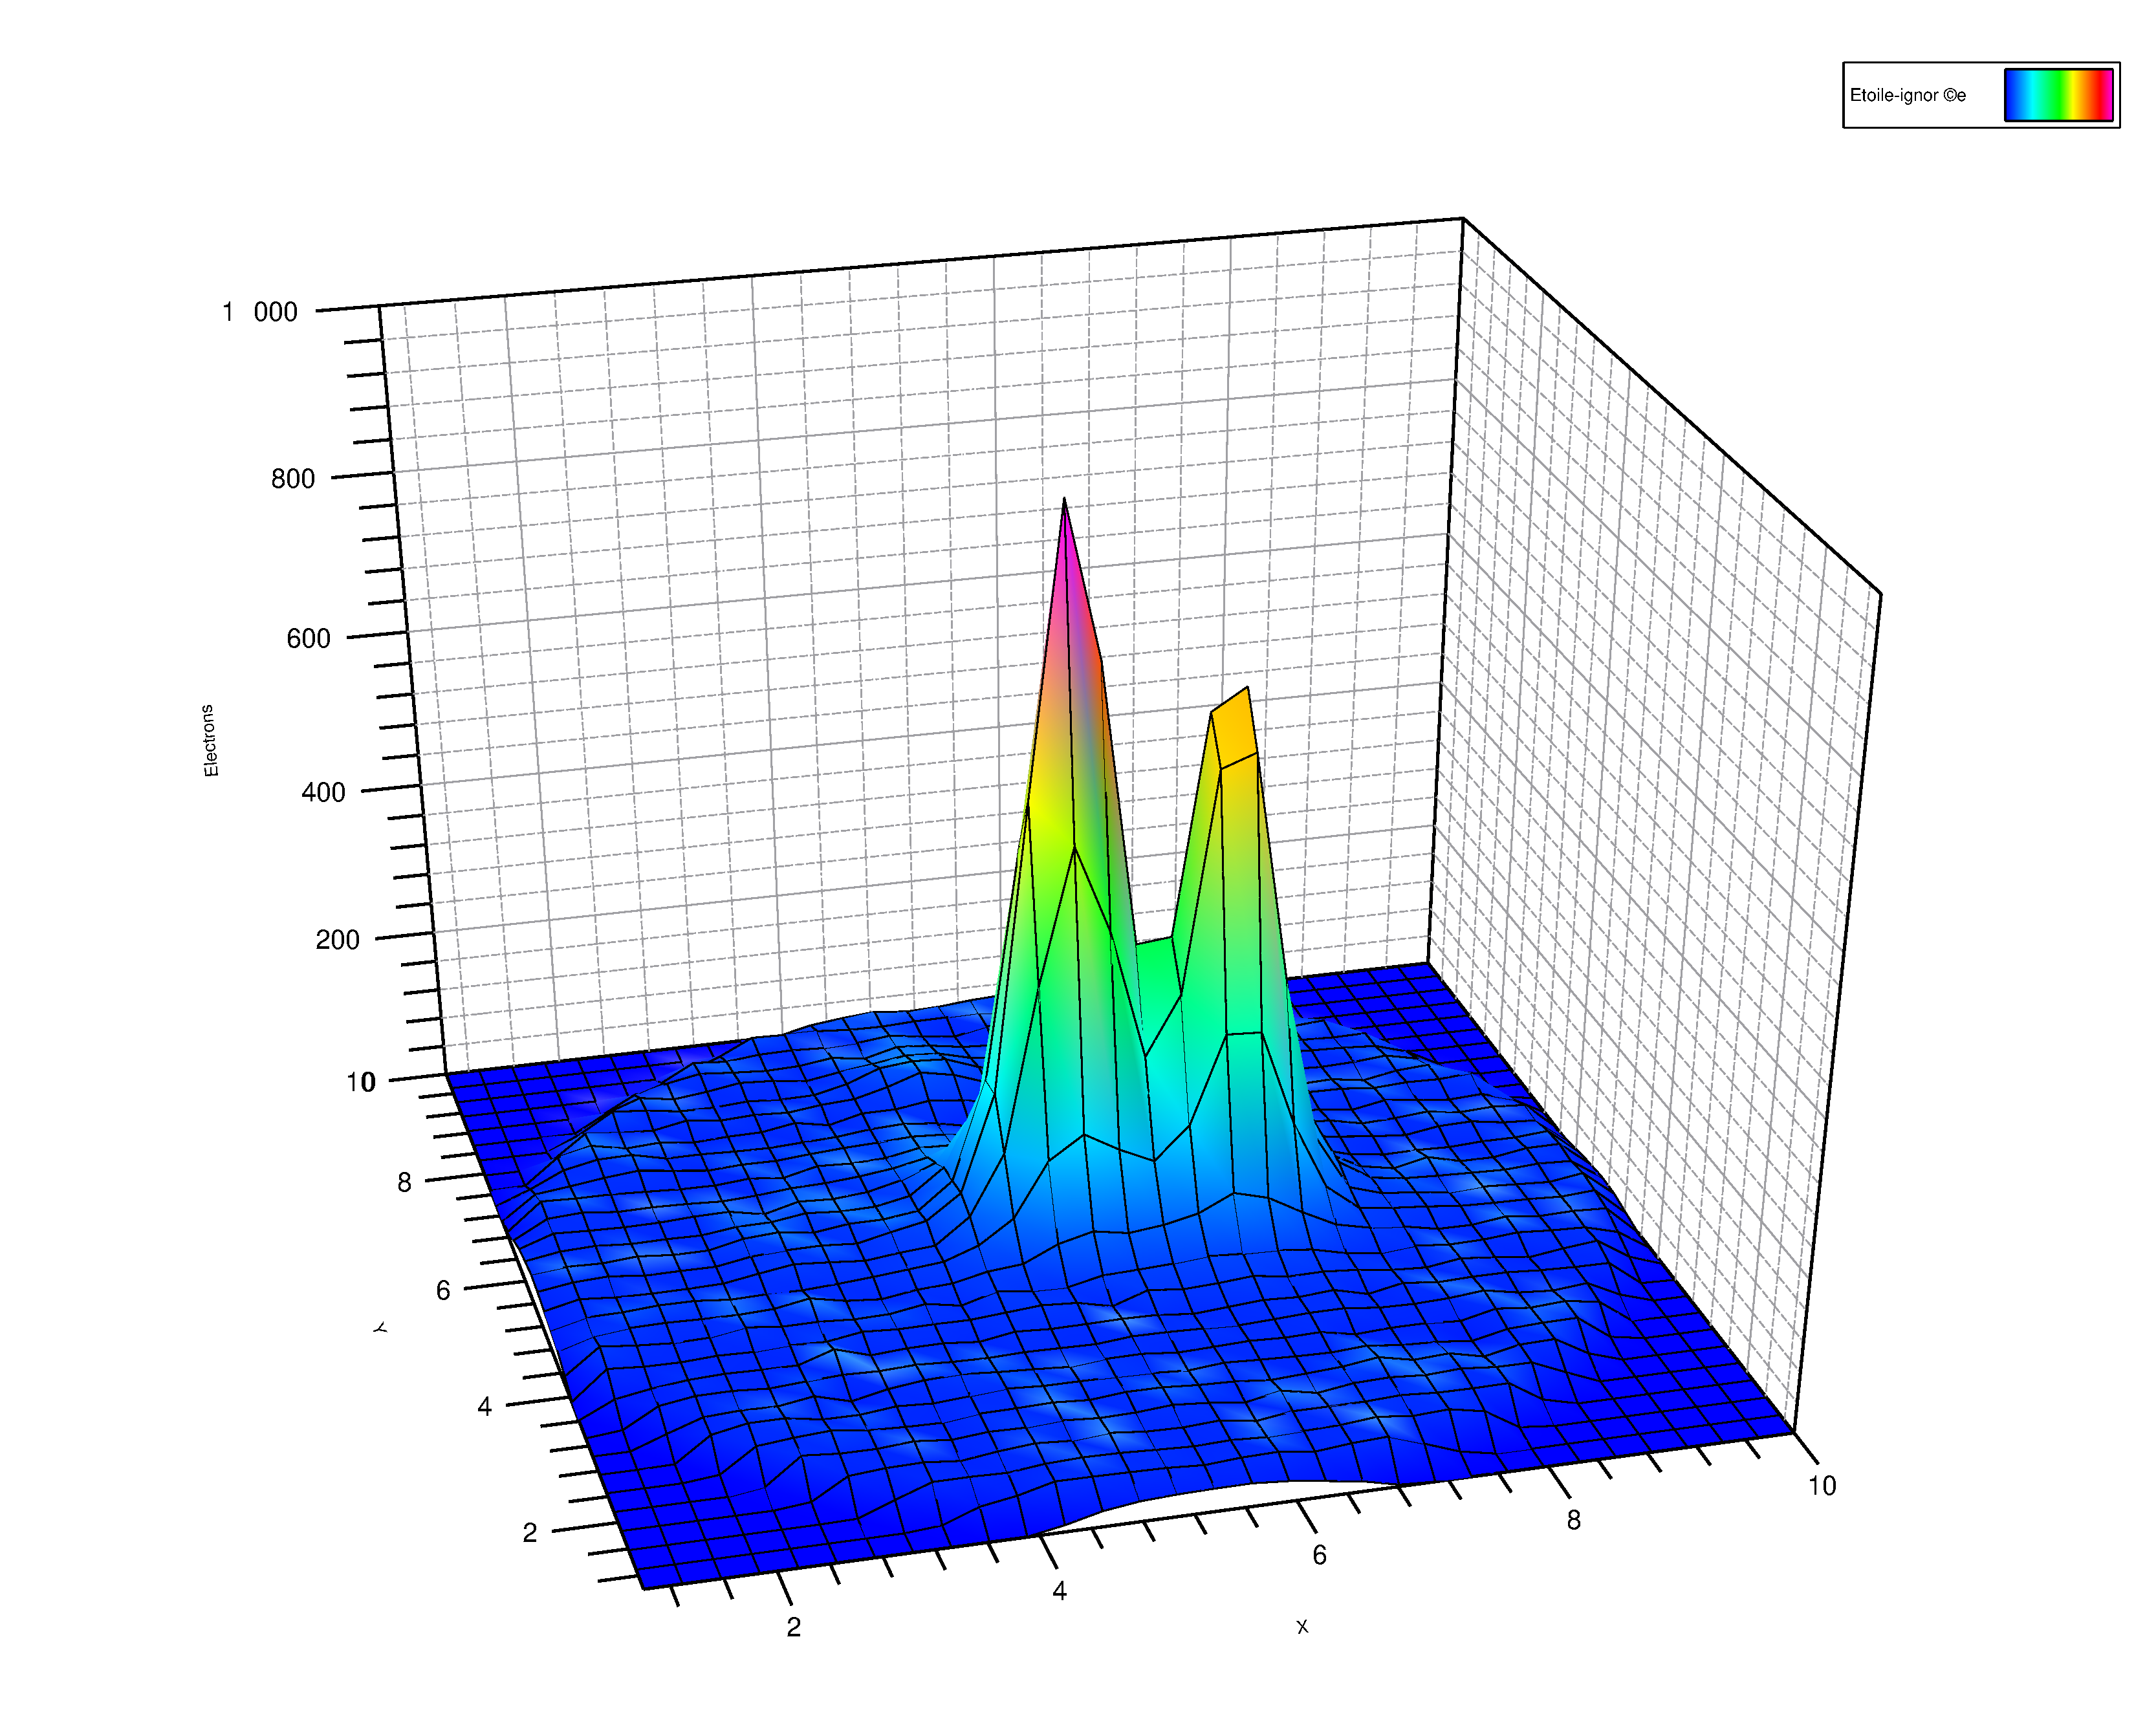
\includegraphics[width=1\textwidth]{fig/etoile ignorée red1.pdf} 
         \label{subfig:excl1}
     \end{subfigure}
     \hfill
          \begin{subfigure}[b]{0.3\textwidth}
              \centering
              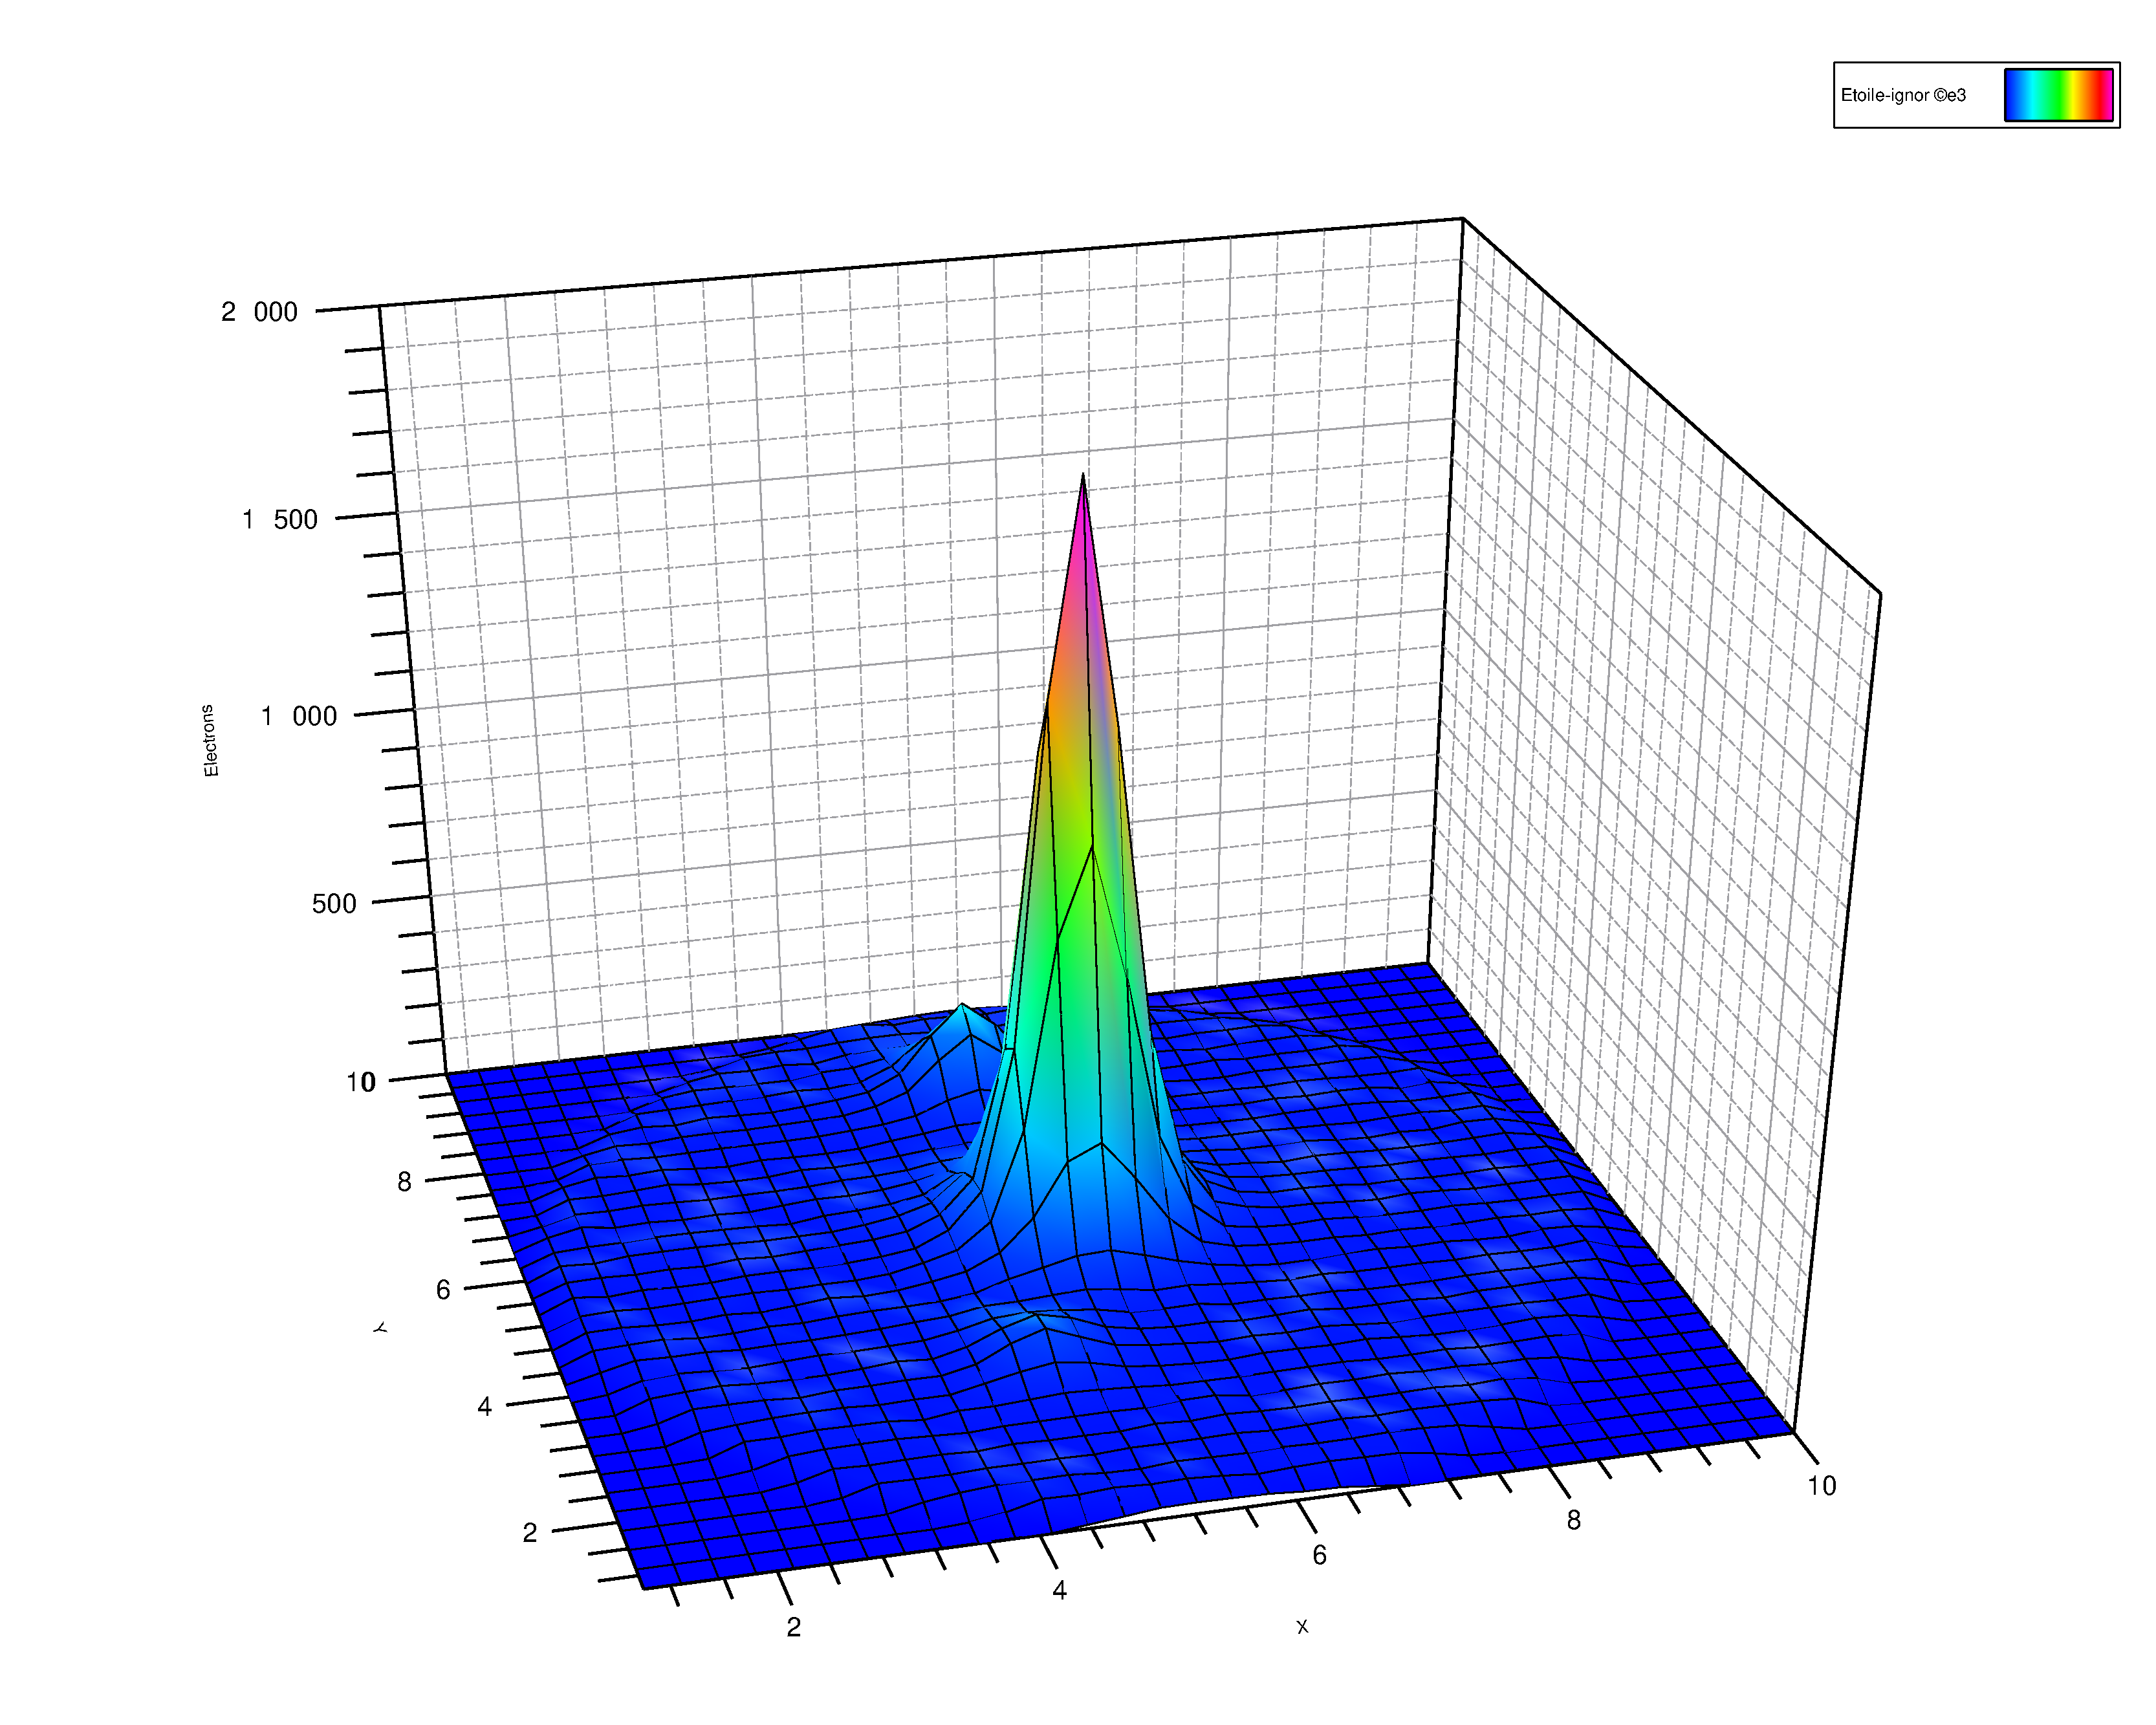
\includegraphics[width=1\textwidth]{fig/etoile ignorée red2.pdf}
              \label{subfig:excl2}
          \end{subfigure}
      \hfill
           \begin{subfigure}[b]{0.3\textwidth}
             \centering
               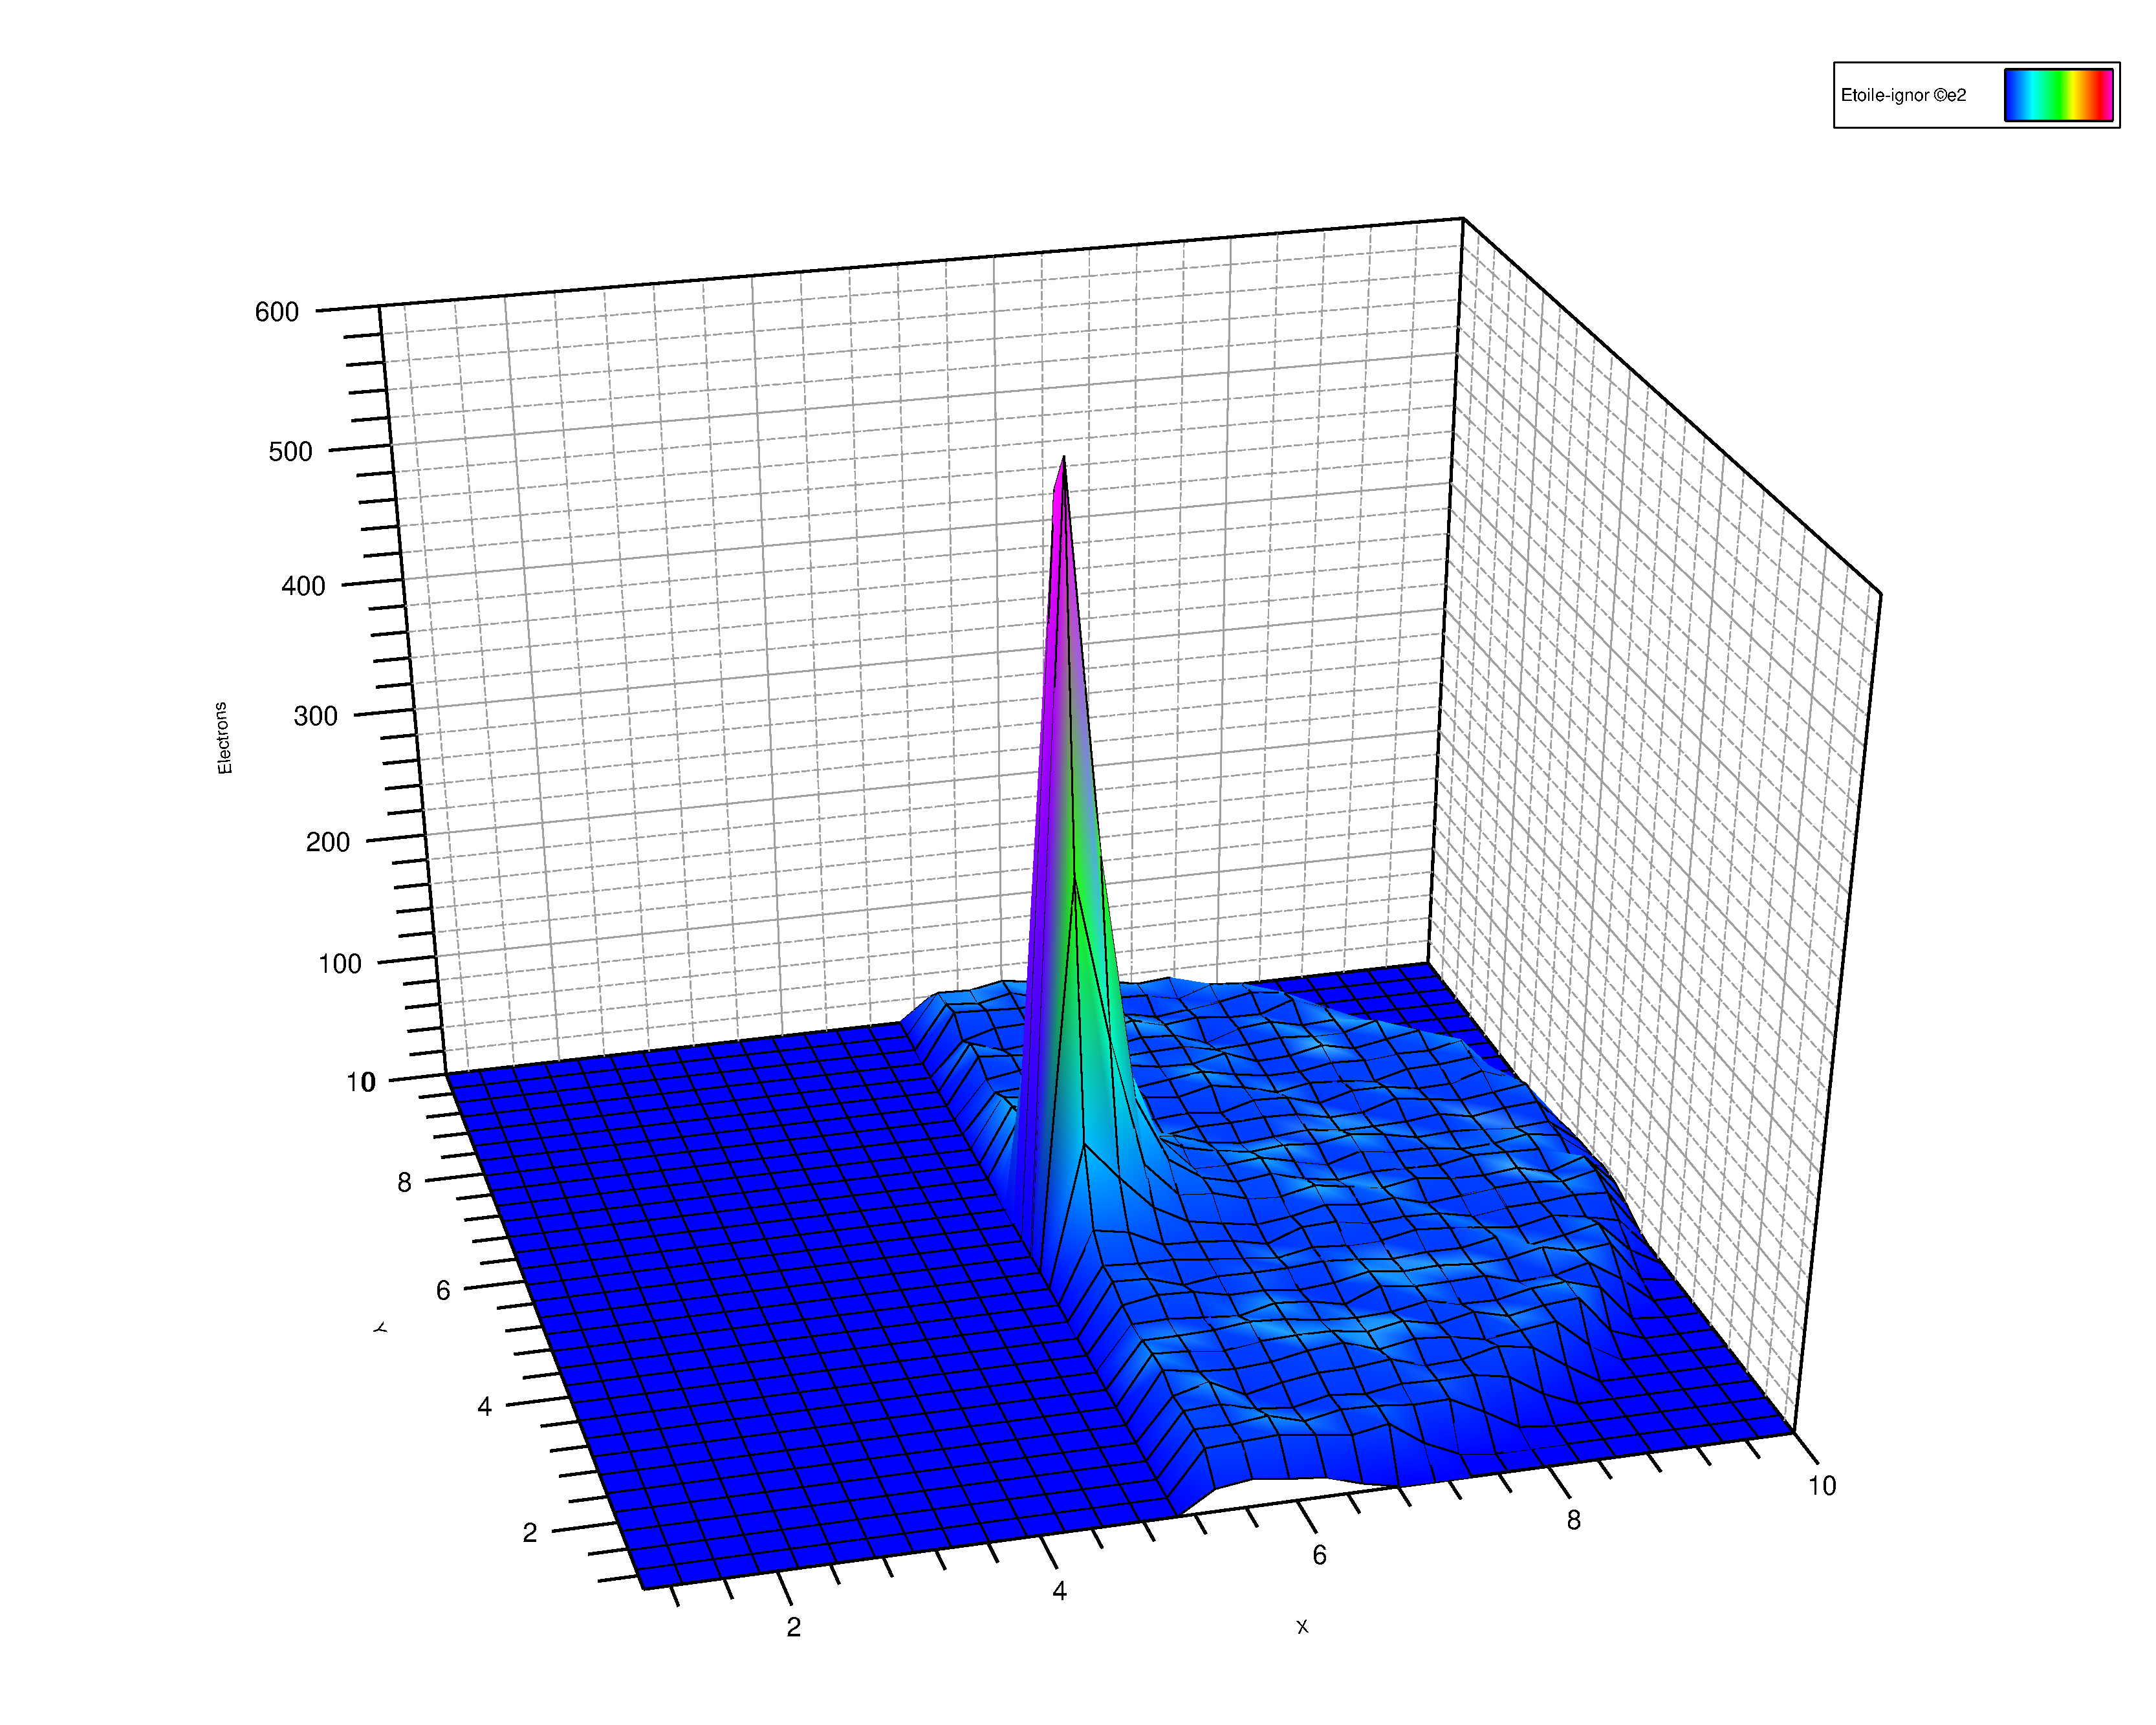
\includegraphics[width=1\textwidth]{fig/etoile ignorée red3.pdf}
               \label{subfig:exlc3}
           \end{subfigure}
           
      \caption{Photons mesurés par le CCD pour trois étoiles écartées de la calibration}
       \label{fig:}
\end{figure}

Les Figures \ref{subfig:excl1} et \ref{subfig:excl2} confortent notre hypothèse: lorsque plusieurs sources sont trop proches, les magnitudes que nous calculons sont erronées car nous n'avons pas de méthode différente de calcul du rayon optimal et du flux pour ces dernières. La Figure \ref{subfig:exlc3} représente un scénario que nous n'avions pas considéré: le cas où la source n'est pas entièrement présente dans le champ.\\

Nous pouvons enfin discuter de la méthode que nous allons retenir pour le rayon d'ouverture optimal. La Figure \ref{subfig:incert corr} nous permet assez facilement d'établir que le critère permettant la calibration la plus précise est celui du critère RSB sur l'étoile avec le pic le plus faible en effet la PSF étant censée être constante à travers notre image ,l'étalement des sources est également constant, ainsi fixer le rayon de cette manière permet d'obtenir un RSB maximal sur toutes les sources sans changer le rayon d'ouverture. Malgré ce dont nous discutions en Section \ref{fluxrsb}, le fait de ne pas mesurer l'entièreté du flux de l'étoile n'est pas un problème dans la mesure où la fraction mesurée est la même pour chaque source, la constante B va donc absorber l'écart que cela induit.\\

Enfin, nous allons observer l'impact des deux méthodes d'annulation du fond de ciel dont nous discutions en Section \ref{méthodes fond} sur l'incertitude de notre zéro de magnitiude, afin de déterminer la mathode optimale. Pour cela, regardons la valeur optimale (fixée à partir de la Figure \ref{subfig:incert corr}) de B pour chaque méthode.

\begin{table}[h]
    \centering
    \begin{tabular}{c|c|c}
         & Fond de ciel global & Fond de ciel local \\
        \hline
        Critère RSB sur chaque source & $23.892 \pm 0.109$ & $23.992 \pm 0.109$ \\
        \hline
        Optimisation RSB/Flux& $23.922 \pm 0.059$ & $23.913 \pm 0.059$\\
        \hline
         Critère RSB sur l'étoile avec le pic le plus faible & $23.811 \pm 0.056$ & $23.811 \pm 0.056$ \\
     \end{tabular}
    \caption{Constante B en fonction des critères utilisés pour fixer les paramètres photométriques (mag) }
    \label{mag}
\end{table}

\noindent Nous pouvons constatons sur la Table \ref{mag} que les variations que nous observions en Figure \ref{subfig:localglobal} n'étaient pas significatives aux échelles de flux que nous considérons ici car elles produisent une incertitude supérieure ou égale sur la constante de calibration aussi nous retiendrons la méthode globale car si celle-ci ne produit pas d'erreur supplémentaire elle reste la plus efficace.

\subsection{Calibration finale\label{cal}}%
  Nous avons désormais déterminé que les paramètres produisant la calibration la plus précise sont une annulation globale de la valeur du fond de ciel avec un rayon d'ouverture fixé par la méthode du RSB de l'étoile au plus faible pic. Nous retiendrons finalement les valeurs suivantes pour le zéro de magnitude pour les filtres r et g, en transposant le raisonnement que l'on vient d'exposer au second filtre. Finalement, nous obtenons:
  \begin{align*}
    &\boxed{B _{r}=23.946 \pm 0.062 \; \text{mag}} &\boxed{B _{g}=23.85 \pm 0.084 \; \text{mag}}
  \end{align*} 
\noindent L'incertitude que nous obtenons pour le second filtre étant plus élevée car à seuil de détection égal, nous détectons moins de sources, or diminuer ce seuil augmente les chances de détecter de "faux positifs" et ajoute des source de faible RSB, cela n'augmente donc pas la précision sur la calibration. 
  
\section{Mesures photométriques et incertitudes}
Maintenant que la calibration photométrique a été effectuée sur nos deux images, nous pouvons procéder à des mesures de magnitudes sur des étoiles en dehors du jeu de données utilisé pour la calibration. Étant donné que nous avons cherché à maximiser le nombre de sources utilisées pour la calibration afin d'en maximiser la précision, nous allons diminuer légèrement le seuil de détection afin de détecter une vingtaine d'étoiles supplémentaires mais dont le RSB ne sera pas aussi optimal que ceux des étoiles du jeu de calibration. Calculons alors leur magnitude à l'incertitude de calibration près et confrontons les aux valeurs de références:

\begin{figure}[h]
     \centering
     \begin{subfigure}[b]{0.4\textwidth}
         \centering
         \includegraphics[width=1\textwidth]{fig/final r.pdf}
         \caption{Filtre r}
         \label{subfig:oui}
     \end{subfigure}
     \hfill
          \begin{subfigure}[b]{0.4\textwidth}
              \centering
              \includegraphics[width=1\textwidth]{fig/final g.pdf}
              \caption{Filtre g}
              \label{subfig:oui2}
          \end{subfigure} 
      \caption{Mesures de magnitudes sur des sources en dehors du jeu de calibration}
       \label{fig:final}
\end{figure}


\noindent Aux incertitudes de calibration près, nous semblons obtenir des magnitudes pertinentes pour la plupart de nos sources en Figure \ref{fig:final}, sauf pour certaines source dont les résultats semblent très loin des valeurs de référence et cela est encore une fois lié à la faible robustesse de notre méthode pour des sources trop proches, si l'on regarde les données du capteur pour les points divergeant de la Figure \ref{subfig:oui} par exemple, nous confirmons cette hypothèse: la Figure \ref{fig:exclu} nous montre encore une fois que dans le cas de sources trop proches les unes des autres, notre méthode de calcul de la magnitude ne produit plus de résultats pertinents.
% Pour les projets de spectroscopie : mesures de longueur d'onde, largeur équivalente, vitesse radiale, identification de raies spectrales
% Pour les projets de photométrie : mesure photométriques sur les étoiles cibles/références
